
\section{Example: A regional model of the Jakobshavn outlet glacier}\label{sec:jako} \index{Jakobshavn} \index{PISM!regional model example}

\optsection{Jakobshavn}

Jakobshavn Isbrae is a fast-flowing outlet glacier in western Greenland that drains approximately 7\% of the area of the Greenland ice sheet, and which has experienced a large acceleration following the loss of its floating tongue in the 1990s \cite{JoughinAbdalatiFahnestock}, an event which seems to have been driven by warmer ocean temperatures \cite{Hollandetal2008}.  Because it is thick, it has a steep surface slope, its flow is significantly defined by bedrock topography, and it has a thick layer of low viscosity temperate ice at its base \cite{Luethietal2009}, this outlet glacier is quite different from the cold, shallow ice streams of West Antarctica \cite{TrufferEchelmeyer}.
 
This Section describes the steps, and the scripts in directory \texttt{examples/jako/}, needed to build a PISM regional model of this outlet glacier.  The same strategy will work for others.  In part, the goal is to allow modest-size computers to run high resolution models, and also large ensembles.\footnote{PISM can do 1km runs for the whole Greenland ice sheet, as shown in this \href{http://www.pism-docs.org/wiki/doku.php?id=news:first1km}{news item}, but you certainly need a supercomputer for that!}  On the other hand, additional data may be available for individual outlet glaciers, and additional model-based analysis is a natural goal.

\index{CReSIS bedrock topography for Jakobshavn}
The geometric data is the SeaRISE 1 km dataset for the whole Greenland ice sheet, which also contains bedrock topography from recent CReSIS radar observations in the Jakobshavn area (\small \url{http://websrv.cs.umt.edu/isis/index.php/1km_Greenland_data_set}\normalsize).  We also use the SeaRISE 5 km data set which has surface mass balance from a atmospheric climate model \cite{Ettemaetal2009}.

\begin{figure}[ht]
  \centering
  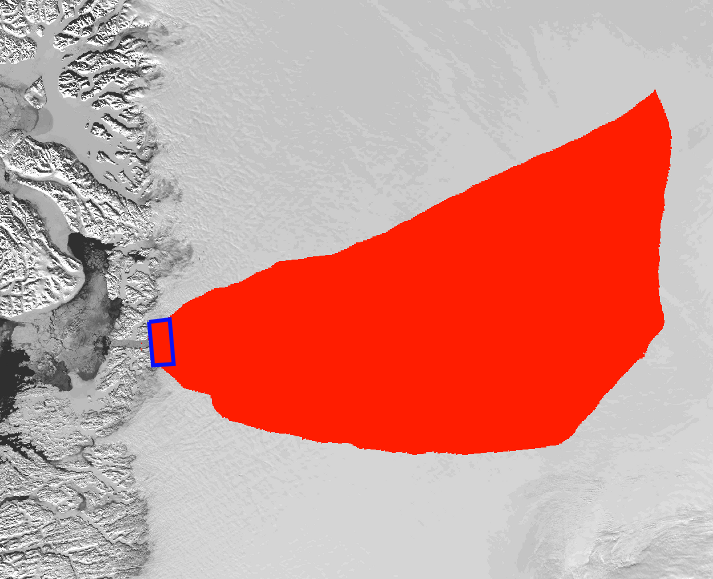
\includegraphics[height=2.1in,keepaspectratio=true]{jako-ftt-mask} \, 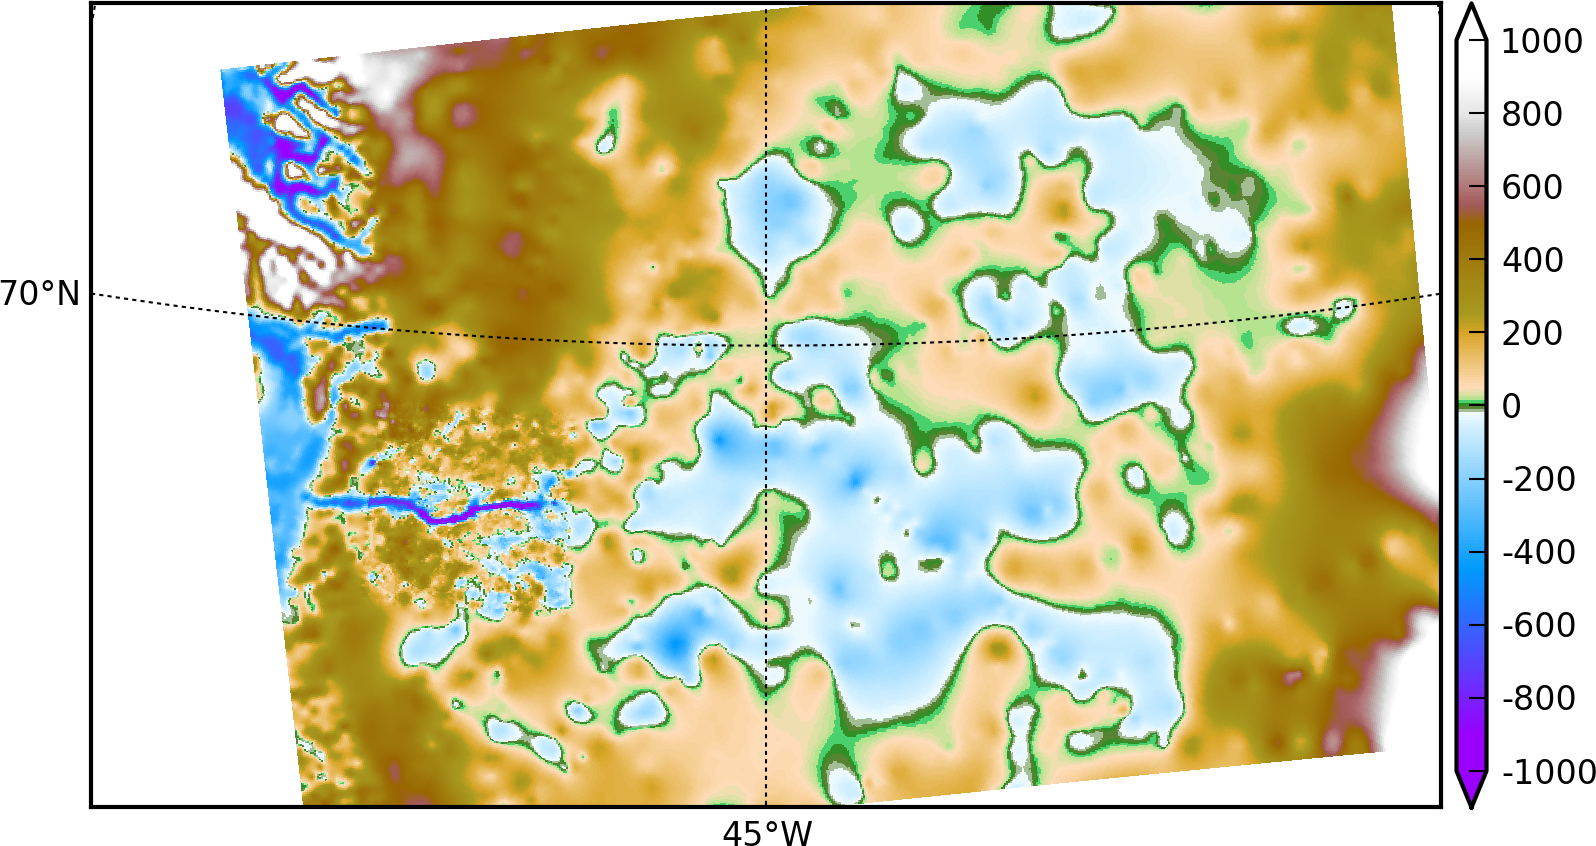
\includegraphics[height=2.1in,keepaspectratio=true]{jako-topg}
  \caption{The Jakobshavn outlet glacier model in this section uses a \texttt{regional-tools} Python script to compute a drainage basin mask from the ice surface elevation (left; Modis background), and starting from a user-identified terminus rectangle (blue).  The regional model benefits from high-resolution bedrock topography in the vicinity of the Jakobshavn fjord (right; scale in meters a.s.l.).}
  \label{fig:jako-basin-topg}
\end{figure}

A regional ice flow model generally needs boundary conditions.  For this we use a 5 km whole ice sheet spun-up model state from PISM, exactly of the type described in Section \ref{sec:start} of this manual.  You can generate the file by running scripts from that Section, or you can download the NetCDF file itself from the PISM website; in fact this download occurs automatically if you run the scripts below.

\index{PISM!pismo executable for outlet glaciers}
\index{regional-tools}
This example in this Section also demonstrates the outlet-glacier-mode PISM executable \texttt{pismo}, and it demonstrates a Python drainage-basin-delineation tool \texttt{regional-tools}, also by the PISM authors, which can be downloaded.

\subsection*{Get the drainage basin delineation tool}
First, get the Python drainage basin generator (using \texttt{git}) and set it up as directed in its \texttt{README.md}.  Then come back to the \texttt{examples/jako/} directory and link to the tool.  Here is the quick summary of these actions:
\begin{quote}\small
\begin{verbatim}
    $ cd ~/usr/local/                                      # the location you want
    $ git clone https://github.com/pism/regional-tools.git
    $ cd regional-tools/
    $ python setup.py install                              # add "--user" to build locally
    $ cd ~/pism/examples/jako/
    $ ln -s ~/usr/local/regional-tools/pism_regional.py .  # symbolic link to tool
\end{verbatim}
\normalsize\end{quote}
To see a description of the drainage basin tool itself, and a bit on how it
works, see \url{https://github.com/pism/regional-tools}.

\subsection*{Preprocess the data and get the whole ice sheet model results}
Next we use a script \texttt{preprocess.sh} that downloads and cleans the 1 km SeaRISE data, an 80 Mb file called \texttt{Greenland1km.nc}.\footnote{If this file is already present then no actual download occurs, and preprocessing proceeds.  So do not worry about download time if you need to preprocess again.  The same comment applies to other downloaded files in this manual.}

The script also downloads the SeaRISE 5 km data set \texttt{Greenland_5km_v1.1.nc}, which contains the surface mass balance model result from RACMO, a field not present in the 1km data set.  If you have already run the example in the first section of this \emph{Manual}, then you already have this file and you can link to it to avoid downloading:
\begin{quote}\small
\begin{verbatim}
    $ ln -s ../searise-greenland/Greenland_5km_v1.1.nc
\end{verbatim}
\normalsize\end{quote}

Finally, the same script also downloads a pre-computed 5 km grid PISM model result \texttt{g5km_0_ftt.nc} for the whole ice sheet.  This is a 1.3Gb file so there may be some delay.  (You can also generate it yourself by running the example in the first section of this \emph{Manual} with its maximum resolution choices, but a supercomputer is recommended for that.)  This download provides the boundary conditions, and the thermodynamical initial condition, for the regional flow model we are building.

So now let's actual run the preprocessing script:
\begin{quote}\small
\begin{verbatim}
    $ ./preprocess.sh
\end{verbatim}
\normalsize\end{quote}
Files \texttt{gr1km.nc}, \texttt{g5km_climate.nc}, and \texttt{g5km_bc.nc} will appear.  These can be examined in the usual ways, for example:
\begin{quote}\small
\begin{verbatim}
    $ ncdump -h gr1km.nc                   # view metadata
    $ ncview gr1km.nc                      # view fields
\end{verbatim}
\normalsize\end{quote}
Note specifically that the boundary condition file \texttt{g5km_bc.nc} contains thermodynamical spun-up variables (\texttt{enthalpy,bmelt,bwat`}) and boundary values for the sliding velocity (\texttt{u_ssa_bc,v_ssa_bc}), which have been extracted from \texttt{g5km_0_ftt.nc}.

None of the above actions is specific to Jakobshavn, though all are specific to the Greenland ice sheet.  If your goal is to build a regional model of another outlet glacier in Greenland, then you may be able to use \texttt{preprocess.sh} immediately.  Note, however, that the SeaRISE 1 km data set only has recent CReSIS bed topography data for the vicinity of the Jakobshavn outlet, and it is otherwise just BEDMAP.  Because outlet glacier flows are bed-topography-dominated, additional effort may be needed to give good models.

\subsection*{Extract the region for modeling}
We are going to extract a ``drainage basin mask'' from the surface elevation data (DEM) in \texttt{gr1km.nc}.  The goal is to determine the locations, outside of the flow into the outlet glacier we want to model, where boundary conditions taken from the precomputed whole ice sheet run can be applied; such locations will be the boundary of the drainage basin.  The basin is determined by the gradient flow from the surface elevation, so, only to determine the extent of our modeled region, we are using a highly-simplified ice dynamics model which says that ice flows down the surface gradient.  Once the drainage basin is determined we will, however, apply the full PISM model in its interior.  Outside the basin we will apply simplified models or use the whole ice sheet results as boundary conditions.

The script \texttt{pism_regional.py} (see above) will identify the drainage basin based on a user choice of a ``terminus rectangle''; see Figure \ref{fig:jako-basin-topg}.  The script can be used in graphical user interface (GUI) mode like this:
\begin{quote}\small
\begin{verbatim}
    $ python pism_regional.py
\end{verbatim}
\normalsize\end{quote}

\noindent\textbf{To use the GUI.}  Select \texttt{gr1km.nc} to open.  Once the topographic map appears in the Figure 1 window, you may zoom enough to see the general outlet glacier area.  Then select the button ``Select terminus rectangle''.  Use the mouse to select a small rectangle around the Jakobshavn terminus (calving front), or around the terminus of another glacier if you want to model that.  Once you have a highlighted rectangle, select a ``border width'' of at least 50 cells.\footnote{This recommendation is somewhat Jakobshavn-specific. We want our model to have an ice-free down flow (western) boundary on the resulting computational domain for the modeled region.}  Then click ``Compute the drainage basin mask.''  Because this is a large data set there will be some delay, but multi-core users will see that an automatic parallel computation is done.  Finally click ``Save the drainage basin mask'' and save with your preferred name; we will assume here that it is ``jakomask.nc.''  Then quit.

\smallskip
\noindent\textbf{To use the command-line interface.}  There are reasons for using the command-line interface of the same script \texttt{pism_regional.py}, including to re-create the mask without changing the terminus rectangle choice, and because of the slowness of the GUI for large data sets.  In fact, for repeatability, we now assume a particular choice of terminus rectangle and we use command-line options to skip the GUI and have the script calculate the drainage basin, as follows:
\begin{quote}\small
\begin{verbatim}
    $ python pism_regional.py -i gr1km.nc -o jakomask.nc -x 360,382 -y 1135,1176 -b 50
\end{verbatim}
\normalsize\end{quote}
This call generated the red region in Figure \ref{fig:jako-basin-topg}.  Options \verb|-x A,B -y C,D| identify the grid indices of the corners of the terminus rectangle, and option \verb|-b| sets the border width.  To see more script options, run with \verb|--help|.

\subsection*{Cut out the computational domain for the regional model}
We still need to ``cut out'', from the whole ice sheet geometry data \verb|gr1km.nc| in particular, the computational domain for the regional model.  (The climate data file \texttt{g5km_climate.nc} and the boundary condition file \texttt{g5km_bc.nc} do not need this action because PISM's coupling and SSA boundary condition code already handles interpolation and/or subsampling for such data.)

You may have noticed that the text output from \texttt{pism_regional.py} includes a cutout command which uses \texttt{ncks} from the NCO tools.  This command also appears as a global attribute of \texttt{jakomask.nc}:
\begin{quote}\small
\begin{verbatim}
    $ ncdump -h jakomask.nc |grep cutout
\end{verbatim}
\normalsize\end{quote}
Copy and run the command that appears, something like
\begin{quote}\small
\begin{verbatim}
    $ ncks -d x,299,918 -d y,970,1394 gr1km.nc jako.nc
\end{verbatim}
\normalsize\end{quote}
This command is also applied to the mask file; note the option \verb|-A| for ``append'':
\begin{quote}\small
\begin{verbatim}
    $ ncks -A -d x,299,918 -d y,970,1394 jakomask.nc jako.nc
\end{verbatim}
\normalsize\end{quote}

Now look at \verb|jako.nc|:
\begin{quote}\small
\begin{verbatim}
    $ ncview -minmax all jako.nc
\end{verbatim}
\normalsize\end{quote}
This file is the full geometry data ready for a regional model.  The field \verb|ftt_mask| still identifies the drainage basin, outside of which we will use simplified time-independent boundary conditions.  Specifically, outside of the \verb|ftt_mask| area, but within the computational domain defined by the extent of \verb|jako.nc|, we will essentially keep the initial thickness.  Inside the \verb|ftt_mask| area all fields will evolve normally.

\subsection*{Spinning-up the regional model on a 5km grid}
All of the above steps, so far in this section, after the first stage of installing and linking to \verb|pism_regional.py|, are accomplished in one script,
\begin{quote}\small
\begin{verbatim}
    $ ./quickjakosetup.sh
\end{verbatim}
\normalsize\end{quote}
Running this takes about a minute on a fast laptop.

To (finally!) run the PISM regional model we will need to know the number of grid points in the 1 km grid in \verb|jako.nc|.  Do this:
\begin{quote}\small
\begin{verbatim}
    $ ncdump -h jako.nc |head
    netcdf jako {
    dimensions:
	  y = 425 ;
	  x = 620 ;
	...
\end{verbatim}
\normalsize\end{quote}
The grid has spacing of 1 km, so our computational domain is a 620 km by 425 km rectangle.  A 2 km resolution, century-scale model run is easily achievable on a desktop or laptop computer, and that is our goal below.  A 5 km resolution spin-up run, matching the resolution of the 5 km whole ice sheet state which was computed on a supercomputer, is also achievable on a small computer, and that is what we do first.

The whole ice sheet model fields in \verb|g5km_bc.nc| may or may not, depending on modeler intent, be spun-up adequately for the purposes of the regional model.  For instance, the intention may be to study equilibrium states with model settings special to the region.  Here we assume that more spin-up is needed.  We will get first an equilibrium 5 km model, and then do a century run of a 2 km model based on the 5 km spin-up.  (Determining ``equilibrium'' requires a decision, of course.  A standard satisfied here is that the ice volume in the region changes by less than 0.1 percent in the final 100 model years.  See \verb|ivol| in \verb|ts_spunjako_0.nc| below.)

Quick calculations for the 5 km grid\footnote{Calculate \texttt{620/5 + 1} and \texttt{425/5 + 1}, for example.} suggest \verb|-Mx 125 -My 86|.  So now we do a basic run using 4 MPI processes:
\begin{quote}\small
\begin{verbatim}
    $ ./spinup.sh 4 125 86 >> out.spin5km &
\end{verbatim}
\normalsize\end{quote}
You can read the script, and watch the run, while it runs:
\begin{quote}\small
\begin{verbatim}
    $ less spinup.sh
    $ less out.spin5km
\end{verbatim}
\normalsize\end{quote}

The run takes about 10 processor-hours.   % 9.12 proc-hours on bueler-lemur
It produces three files which can be viewed (e.g.~with \verb|ncview|): \verb|spunjako_0.nc|, \verb|ts_spunjako_0.nc|, and \verb|ex_spunjako_0.nc|.

Generally the regridding techniques used at the start of this run are recommended for regional modeling.  In fact, some more comments are appropriate:
\begin{itemize}
\item  We use \verb|-boot_file| on \verb|jako.nc|, so we get to choose our grid, and (as usual in PISM with \verb|-boot_file|) the fields are interpolated to our grid.  A modestly-fine vertical grid with 20 m spacing is chosen, but even finer is recommended, especially to resolve the temperate ice layer in these outlet glaciers.
\item There is option \verb|-no_model_strip 10| asking \verb|pismo| to put a 10 km strip around edge of the computational domain; in this strip some variables will be held fixed.  Specifically the thermodynamical spun-up variables \verb|enthalpy,bmelt,bwat| from \verb|g5km_bc.nc| are held fixed and used as boundary conditions for the conservation of energy model in the strip. (An alternative is to have the enthalpy and other thermodynamical variables not spun-up at all in the strip, which would happen if options \verb|-regrid_...| were not used.  However, the resulting not-very-realistic ice temperatures and softness/hardness is advected inward.)
\item Dirichlet boundary conditions \verb|u_ssa_bc,v_ssa_bc| are read for the sliding stress balance (the SSA) from the same file.  The SSA equations are solved as usual other than in the \verb|no_model_strip| where these Dirichlet boundary conditions are used.  (An alternative for the SSA boundary conditions is to have zero velocity in the \verb|no_model_strip|, but the velocity tangent to the north and south edges of the strip is significantly nonzero in fact.)
\item The calving front of the glacier is handled by the following option combination:

  \verb|-ocean_kill file.nc -cfbc -kill_icebergs|
  
\noindent This choice uses the present-day ice extent to determine the location of the calving front, but it then applies the PIK mechanisms for the stress boundary condition at the calving front (\verb|-cfbc|) and it uses \verb|-kill_icebergs| to eliminate any stray floating pieces of ice (for which stress balances are ill-posed \cite{Winkelmannetal2011}).
\end{itemize}

\subsection*{Century run on a 2km grid}
Now that we have a spun-up state, here is a 100 model year run on a 2km grid:
\begin{quote}\small
\begin{verbatim}
    $ ./century.sh 4 311 213 spunjako_0.nc >> out.2km_100a &
\end{verbatim}
\normalsize\end{quote}
This run requires at least 6 Gib of memory, and it takes about 20 processor-hours. % 17.77 proc-hours on bueler-lemur

It produces a file almost immediately, namely \verb|jakofine_short.nc|, and then restarts from it.  This is explained by the need to regrid fields first from the result of the previous 5 km regional run, i.e. from \verb|spunjako_0.nc|, and then to ``go back'' and regrid the SSA boundary conditions from the 5 km whole ice sheet results, i.e.~from the file \verb|g5km_bc.nc|.

At the end of the run the final file \verb|jakofine.nc| is produced, along with a time-series result file \verb|ts_jakofine.nc| with monthly scalar time-series, and a spatial time-dependent result file |ex_jakofine.nc|.  The latter is a source of simple ``movies'' of the simulation.  Note that the flow does not appear to reach a steady state, even though the climate forcing and boundary conditions are time-independent.  The surface speed at the end of this run is shown in Figure \ref{fig:jako-csurf}, with a comparison to the observations.

\begin{figure}[ht]
  \centering
  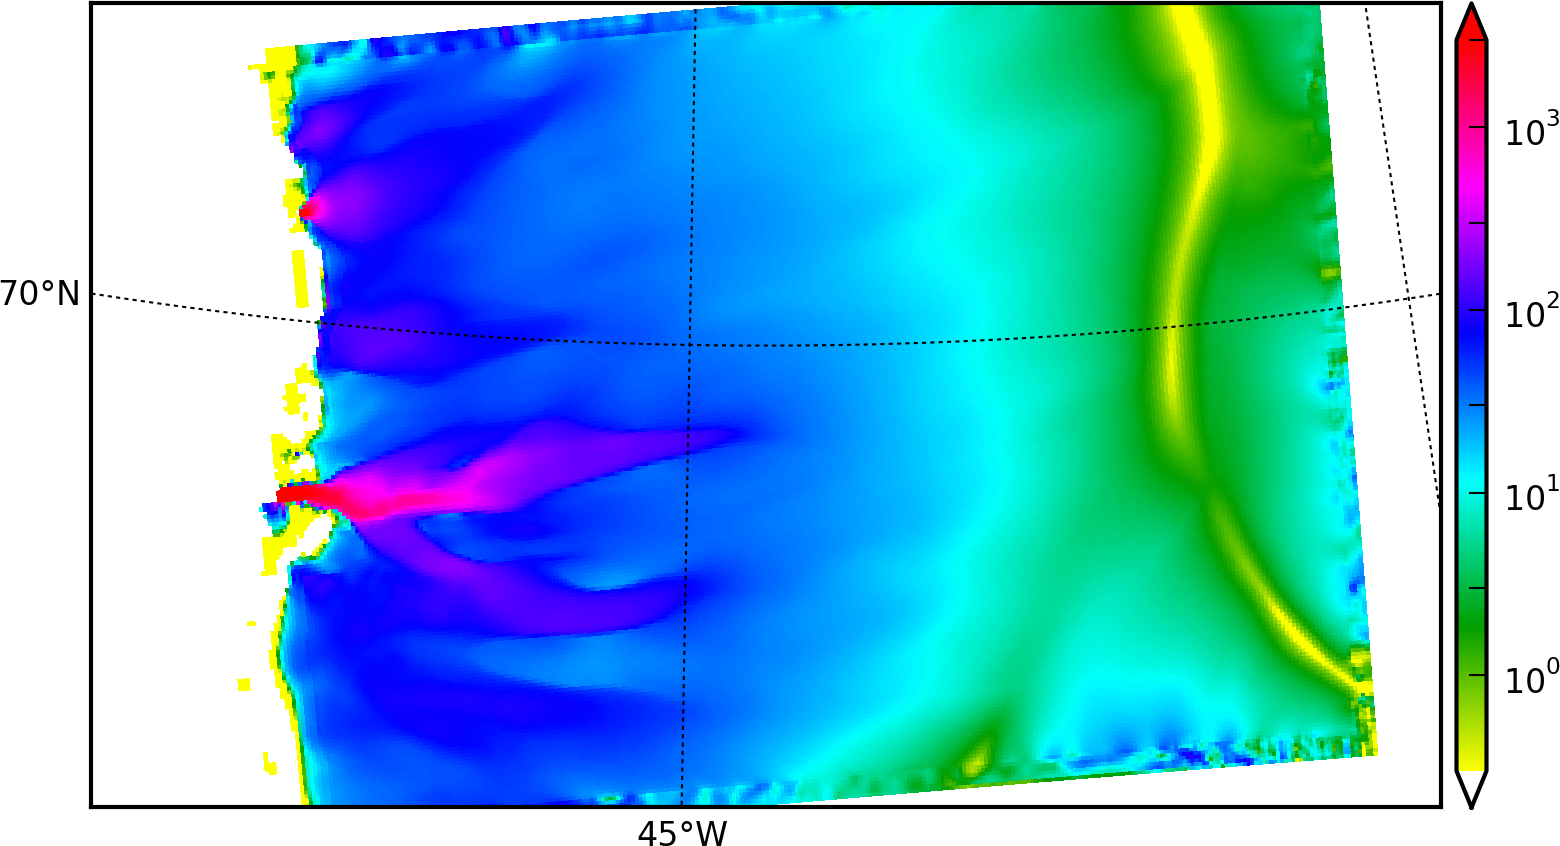
\includegraphics[height=1.8in,keepaspectratio=true]{jako-csurf} \, 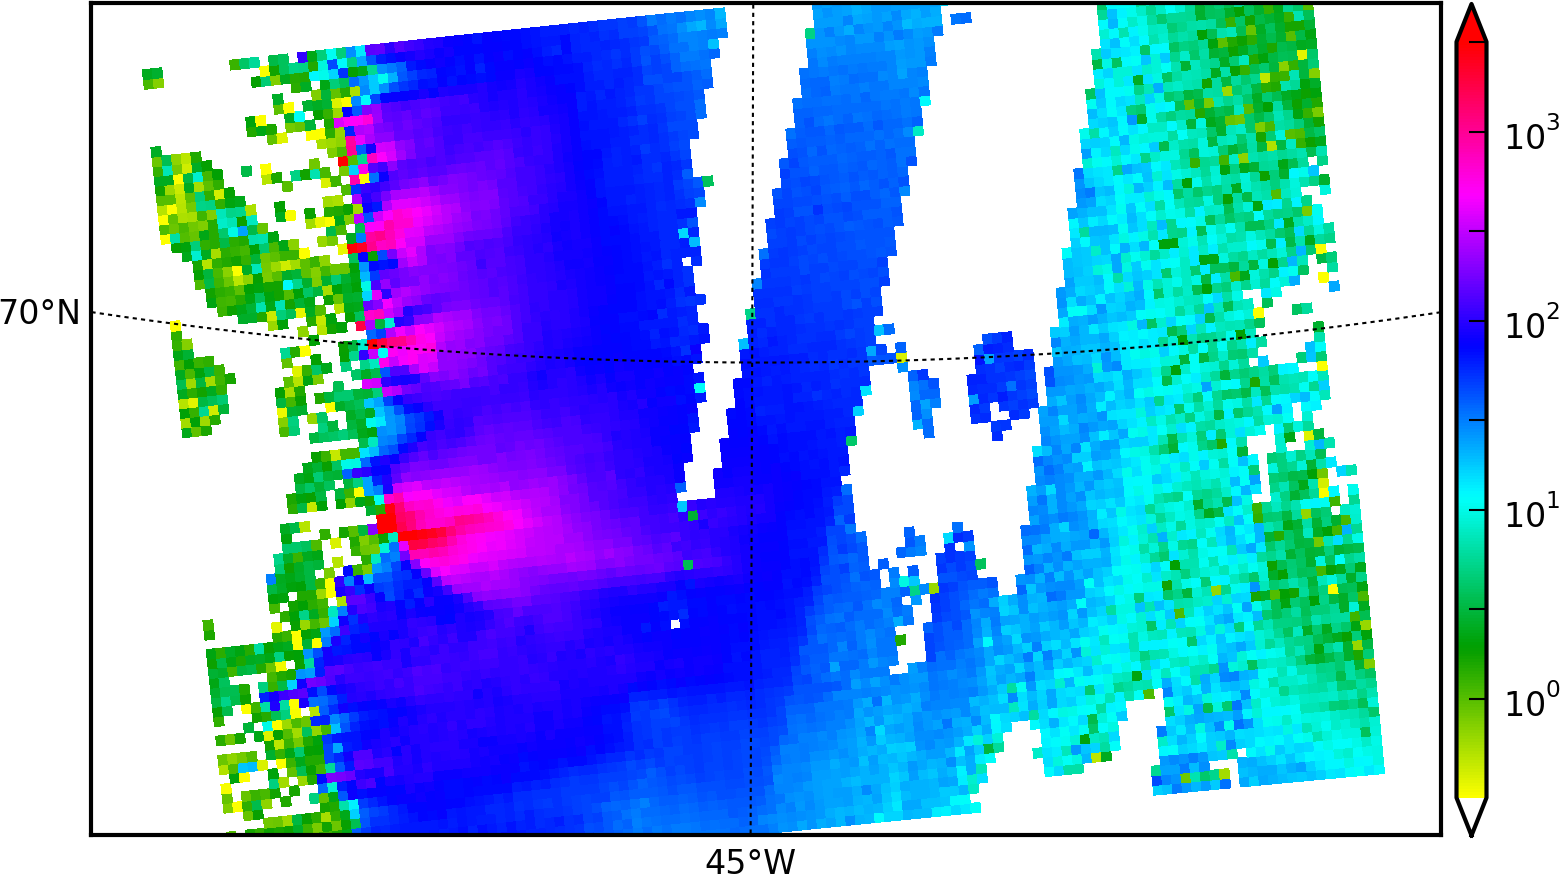
\includegraphics[height=1.8in,keepaspectratio=true]{jako-surfvelmag-true}
  \caption{The modeled surface speed at the end of a 100 model year, 2 km grid run (left; FIXME: it is a place-holder generated from \texttt{jakofine_short.nc}!).  Observed surface speed from the SeaRISE  5 km data set (right), for a similar region.  Scales are in meters per year.}
  \label{fig:jako-csurf}
\end{figure}


\begin{comment}

\subsection*{Plotting the results}

This is about Figure {fig:jako-csurf}.  We use  PyPISMTools.

To visualize the surface speed at the end of the 2km run, download PyPISMTools and do

  basemap-plot.py --singlerow -v csurf -o csurf.png jakofine.nc

To choose a colormap add option \verb|--colormap foo.cpt| or similar; some colormaps can 

  cp Greenland_5km_v1.1.nc gr5km_xy.nc
  ncrename -v x1,x -v y1,y gr5km_xy.nc 
  ncrename -d x1,x -d y1,y gr5km_xy.nc 
  ncks -d x,55,175 -d y,195,280 -v lat,lon,mapping,surfvelmag gr5km_xy.nc foo.nc
  basemap-plot.py --singlerow -v surfvelmag -o surfvelmag.png foo.nc

\end{comment}